% This file requires the following packages in your preamble:
% \usepackage{graphicx}
% \usepackage{adjustbox}
% \usepackage{placeins}

% Introduction figures - Project moodboards and artistic vision
% PLACEMENT: Einführung.tex - Show project aesthetics and artistic direction for "Echoes of the Mind"
\FloatBarrier
\begin{figure}[htbp]
    \centering
    \adjustbox{max width=0.9\textwidth, max height=0.8\textheight, keepaspectratio}{%
        \includegraphics{images/docupictures/EchoesOfTheMind_startbild.png}%
    }
    \caption{MoodBoard-Startbild des Projektes \glqq Echoes of the Mind\grqq{}}
    \label{fig:echoes_startbild}
\end{figure}

% PLACEMENT: Einführung.tex - Emotional visualization concepts showing artistic collaboration context
\begin{figure}[htbp]
    \centering
    \adjustbox{max width=0.9\textwidth, max height=0.8\textheight, keepaspectratio}{%
        \includegraphics{images/docupictures/EchoesOfTheMind_mood.png}%
    }
    \caption{Künstlerische Vision: Emotionale Visualisierungskonzepte für \glqq Echoes of the Mind\grqq{}}
    \label{fig:echoes_mood}
\end{figure}

% Sprint 1 figures - Initial system design (later deprecated)
% PLACEMENT: Entwicklungsprozess.tex - Show early dual-source approach before architectural simplification
\FloatBarrier
\begin{figure}[htbp]
    \centering
    \adjustbox{max width=0.9\textwidth, max height=0.85\textheight, keepaspectratio}{%
        \includegraphics{images/docupictures/MASK.png}%
    }
    \caption{Anfängliches Systemdesin von M.A.S.K. mit Analyse- und Triggerprozess und dem später nach Sprint 2 deprecated Dual-Source-Ansatz}
    \label{fig:mask_architecture}
\end{figure}

% Sprint 2 figures - MediaPipe skeleton foundation
% PLACEMENT: stand_der_technik.tex - Explain MediaPipe node structure as technical basis for tracking
\FloatBarrier
\begin{figure}[htbp]
    \centering
    \adjustbox{max width=0.9\textwidth, max height=0.8\textheight, keepaspectratio}{%
        \includegraphics{images/docupictures/mediapipeNODES.png}%
    }
    \caption{MediaPipe Skeleton-Nodes, die die Basis für die Skelett-Visualisierung bilden}
    \label{fig:mediapipe_nodes}
\end{figure}

% PLACEMENT: Entwicklungsprozess.tex - Show deprecated Kinect approach before MediaPipe-only solution
\begin{figure}[htbp]
    \centering
    \adjustbox{max width=0.7\textwidth, max height=0.8\textheight, keepaspectratio}{%
        \includegraphics{images/docupictures/kinect_nodes.png}%
    }
    \caption{Kinect V2 Skeleton-Visualisierung mit Node-Nummerierung | Vor Sprint 2 mit MediaPipe Nodes gemischt mit Mapping, später deprecated}
    \label{fig:kinect_nodes}
\end{figure}

% PLACEMENT: Sprint2.tex or Entwicklungsprozess.tex - Development and testing phase
\begin{figure}[htbp]
    \centering
    \adjustbox{max width=0.9\textwidth, max height=0.6\textheight, keepaspectratio}{%
        \includegraphics{images/docupictures/KinectMediaPipe_Testing.png}%
    }
    \caption{TouchDesigner Testing-Interface: Unterschied zwischen der Mediapipe Skeleton-Visualisierung (oben, pink) und der Kinect V2 Skeleton-Visualisierung (unten, grün)}
    \label{fig:testing_interface}
\end{figure}

% Sprint 3 figures
% PLACEMENT: Sprint3.tex - Design concepts and scaling solutions
\FloatBarrier
\begin{figure}[htbp]
    \centering
    \adjustbox{max width=0.8\textwidth, max height=0.8\textheight, keepaspectratio}{%
        \includegraphics{images/docupictures/Sprint3_1.jpg}%
    }
    \caption{Erstes künsterlisches Konzept der Blobs: Blobs sind magnetisch anziehend/abstoßend zum Künstler}
    \label{fig:scaling_concept}
\end{figure}

% PLACEMENT: Sprint3.tex - Spatial distribution concepts
\begin{figure}[htbp]
    \centering
    \adjustbox{max width=0.8\textwidth, max height=0.8\textheight, keepaspectratio}{%
        \includegraphics{images/docupictures/Sprint3_2.jpg}%
    }
    \caption{Künsterlisches Konzept, das übernommen wurde: Je nach Position des Performers werden die Blobs krisselig/blitzig oder ruhig dargestellt)}
    \label{fig:external_positioning}
\end{figure}

% PLACEMENT: Sprint3.tex - Interaction design concepts
\begin{figure}[htbp]
    \centering
    \adjustbox{max width=0.8\textwidth, max height=0.8\textheight, keepaspectratio}{%
        \includegraphics{images/docupictures/Sprint3_3.jpg}%
    }
    \caption{Künsterlisches Konzept, das deprecated wurde, nachdem meine Shader-Solution nicht geklappt hatte: Magnetische Interaktion: Dynamische Visual-Performer-Relation}
    \label{fig:magnetic_interaction}
\end{figure}

% PLACEMENT: Sprint3.tex - Movement-responsive system design
\begin{figure}[htbp]
    \centering
    \adjustbox{max width=0.6\textwidth, max height=0.8\textheight, keepaspectratio}{%
        \includegraphics{images/docupictures/Sprint3_4.jpg}%
    }
    \caption{Künsterlisches Konzept, das übernommen wurde: der Performer ist in einem hellen Kreis, und bewegt sich}
    \label{fig:movement_responsive}
\end{figure}

% PLACEMENT: Sprint3.tex - Composite effect concepts
\begin{figure}[htbp]
    \centering
    \adjustbox{max width=0.8\textwidth, max height=0.8\textheight, keepaspectratio}{%
        \includegraphics{images/docupictures/Sprint3_5.jpg}%
    }
    \caption{Künsterlisches Konzept, das übernommen wurde: der Performer ist in einem hellen Kreis, und die Visuals brechen interaktiv mit seinen Extremitäten-Koordinaten passend aus}
    \label{fig:composite_effects}
\end{figure}

% Sprint 5 figures
% PLACEMENT: Systemarchitektur_und_Ergebnisse.tex or Sprint5.tex - Main system interface
\FloatBarrier
\begin{figure}[htbp]
    \centering
    \adjustbox{max width=0.9\textwidth, max height=0.8\textheight, keepaspectratio}{%
        \includegraphics{images/docupictures/Finished_MediaPipeContainer_mitErklärungen.png}%
    }
    \caption{M.A.S.K. MediaPipe-Container: Alle modules des Containers mit Erklärungen (farblich markiert)}
    \label{fig:main_interface}
\end{figure}

% PLACEMENT: Systemarchitektur_und_Ergebnisse.tex - Technical implementation details
\begin{figure}[htbp]
    \centering
    \adjustbox{max width=0.9\textwidth, max height=0.8\textheight, keepaspectratio}{%
        \includegraphics{images/docupictures/NodeXYzuSOPZentriertemTranslate.png}%
    }
    \caption{Koordinatentransformation der Hand-Feuer-Visualisierung: Node-XY zu zentralisiertem SOP-Translate}
    \label{fig:coordinate_transformation}
\end{figure}

% PLACEMENT: Sprint4.tex or Demonstration.tex - Visual effect implementation
\begin{figure}[htbp]
    \centering
    \adjustbox{max width=0.9\textwidth, max height=0.8\textheight, keepaspectratio}{%
        \includegraphics{images/docupictures/NoisyBlob_animatedSwitchzwischenBlitzUndNichtBlitzBeiTrackingTrigger.png}%
    }
    \caption{NoisyBlob Adaptive Visual-Switch: Animierte Zustandsmaschine mit Tracking-Triggern anhand der Spine-Base zu Händen-Position mit Smooth Transition zwischen Blitz und Nicht-Blitz}
    \label{fig:animated_switch}
\end{figure}

% PLACEMENT: Sprint5.tex or Systemarchitektur_und_Ergebnisse.tex - Core pipeline implementation
\begin{figure}[htbp]
    \centering
    \adjustbox{max width=0.9\textwidth, max height=0.8\textheight, keepaspectratio}{%
        \includegraphics{images/docupictures/NoisyBlob_HEAD_to_ParticleGPU_Translate.png}%
    }
    \caption{NoisyBlob ParticleGPU-Pipeline: Head-Node zu ParticleGPU Translation mit Transformation von Mediapipe zu Center-Offsets}
    \label{fig:particle_translation}
\end{figure}

% PLACEMENT: Sprint6.tex or Systemarchitektur_und_Ergebnisse.tex - 64-spike system mathematics
\begin{figure}[htbp]
    \centering
    \adjustbox{max width=0.8\textwidth, max height=0.8\textheight, keepaspectratio}{%
        \includegraphics{images/docupictures/TopDown_KreisZuRampsParametisierteBerechnungen.png}%
    }
    \caption{64-Spike Radialsystem im Testing: Polar-Koordinaten-Berechnung mit parametrisierter Ramp-Generation, hier mit erklärenden farblichen Texten zu den einzelnen Modulen}
    \label{fig:radial_spike_system}
\end{figure}

% Ausfuehrungsdokumentation figures
% PLACEMENT: Ausfuehrungsdokumentation.tex - Production environment setup
\FloatBarrier
\begin{figure}[htbp]
    \centering
    \adjustbox{max width=0.8\textwidth, max height=0.8\textheight, keepaspectratio}{%
        \includegraphics{images/onSetImages/InsideWideshotAlbrechtAdeStudio.jpg}%
    }
    \caption{Albrecht-Ade-Studio: Eindrücke der großen Soundstage nach den zwei Drehtagen. Das Studio wirkt wie leergefegt.}
    \label{fig:studio_interior}
\end{figure}

% PLACEMENT: Ausfuehrungsdokumentation.tex - Technical operation during production
\begin{figure}[htbp]
    \centering
    \adjustbox{max width=0.7\textwidth, max height=0.8\textheight, keepaspectratio}{%
        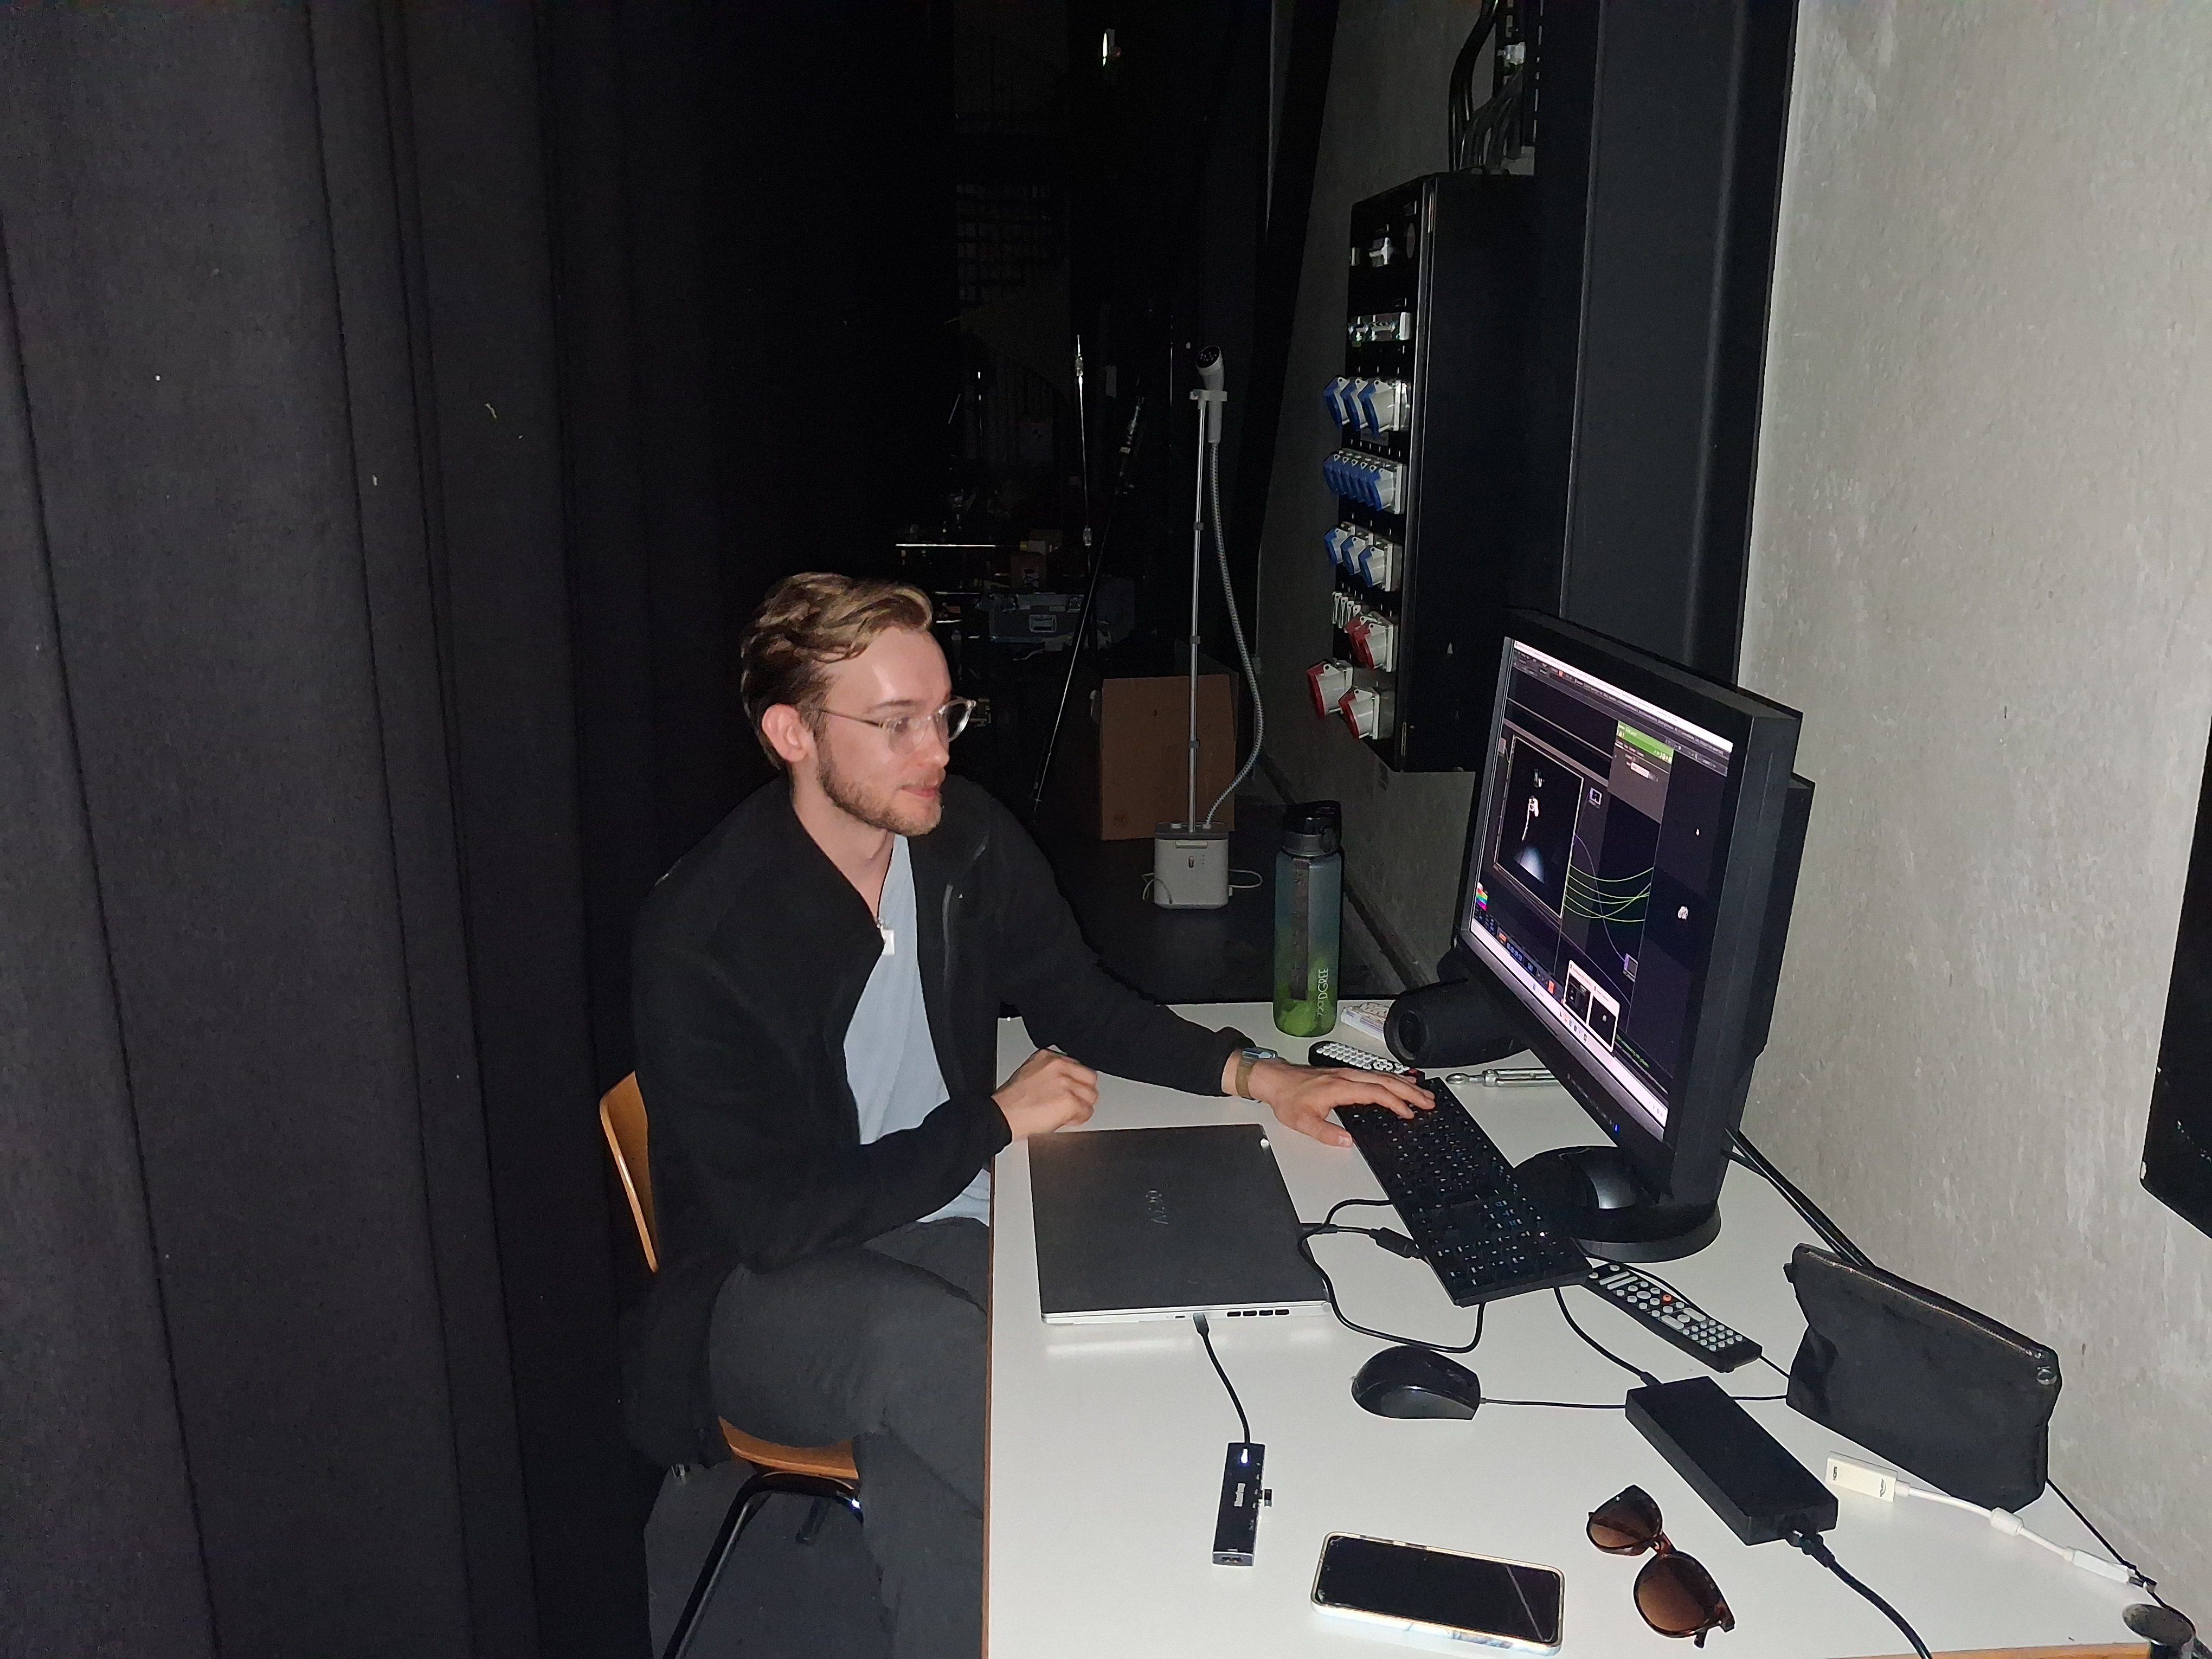
\includegraphics{images/onSetImages/MartyBehindTheStudioCurtainDoingTouchDesigner.jpg}%
    }
    \caption{Technische Umsetzung: TouchDesigner-Bedienung hinter dem Studievorhang während der Produktion}
    \label{fig:technical_operation}
\end{figure}

% PLACEMENT: Ausfuehrungsdokumentation.tex - Production preparation and setup
\begin{figure}[htbp]
    \centering
    \adjustbox{max width=0.7\textwidth, max height=0.8\textheight, keepaspectratio}{%
        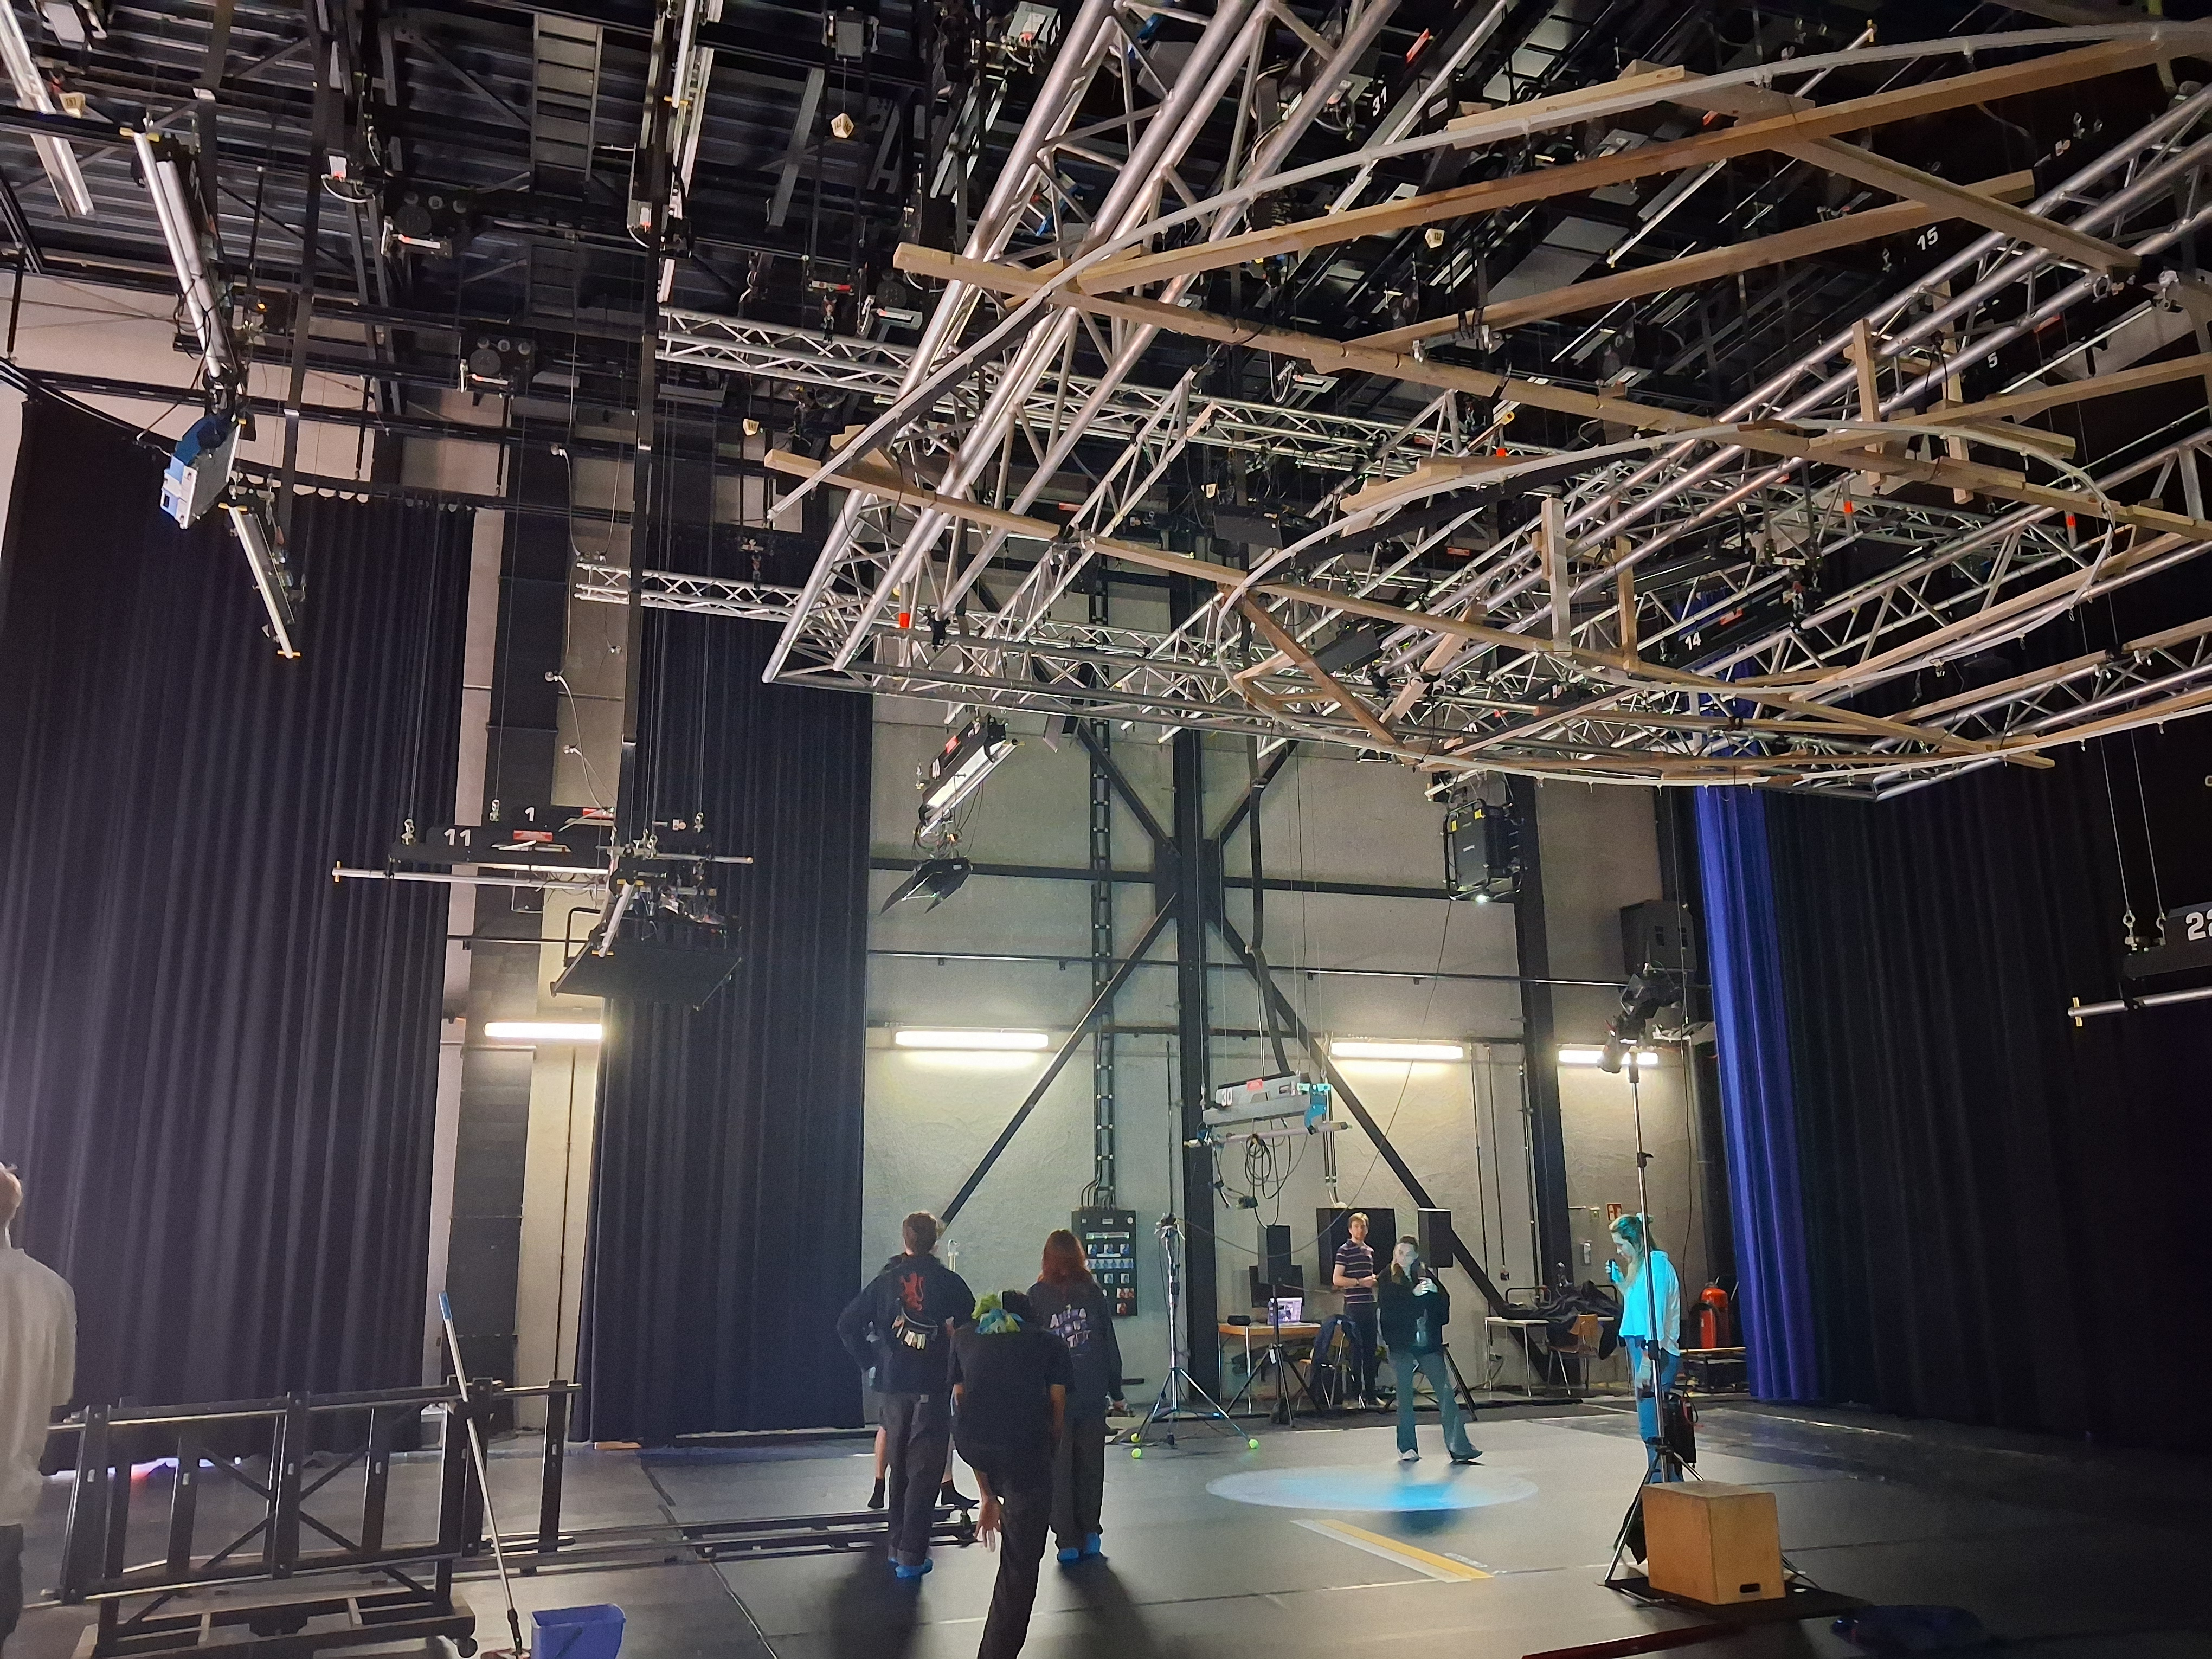
\includegraphics{images/onSetImages/wideStudioShotPreparingTopDownSpikeShot.jpg}%
    }
    \caption{Studio-Vorbereitung: Setup für Top-Down-Spike-System mit Overhead-Kamera-Positionierung}
    \label{fig:topdown_setup}
\end{figure}

% PLACEMENT: Ausfuehrungsdokumentation.tex - Production monitoring and results
\begin{figure}[htbp]
    \centering
    \adjustbox{max width=0.7\textwidth, max height=0.8\textheight, keepaspectratio}{%
        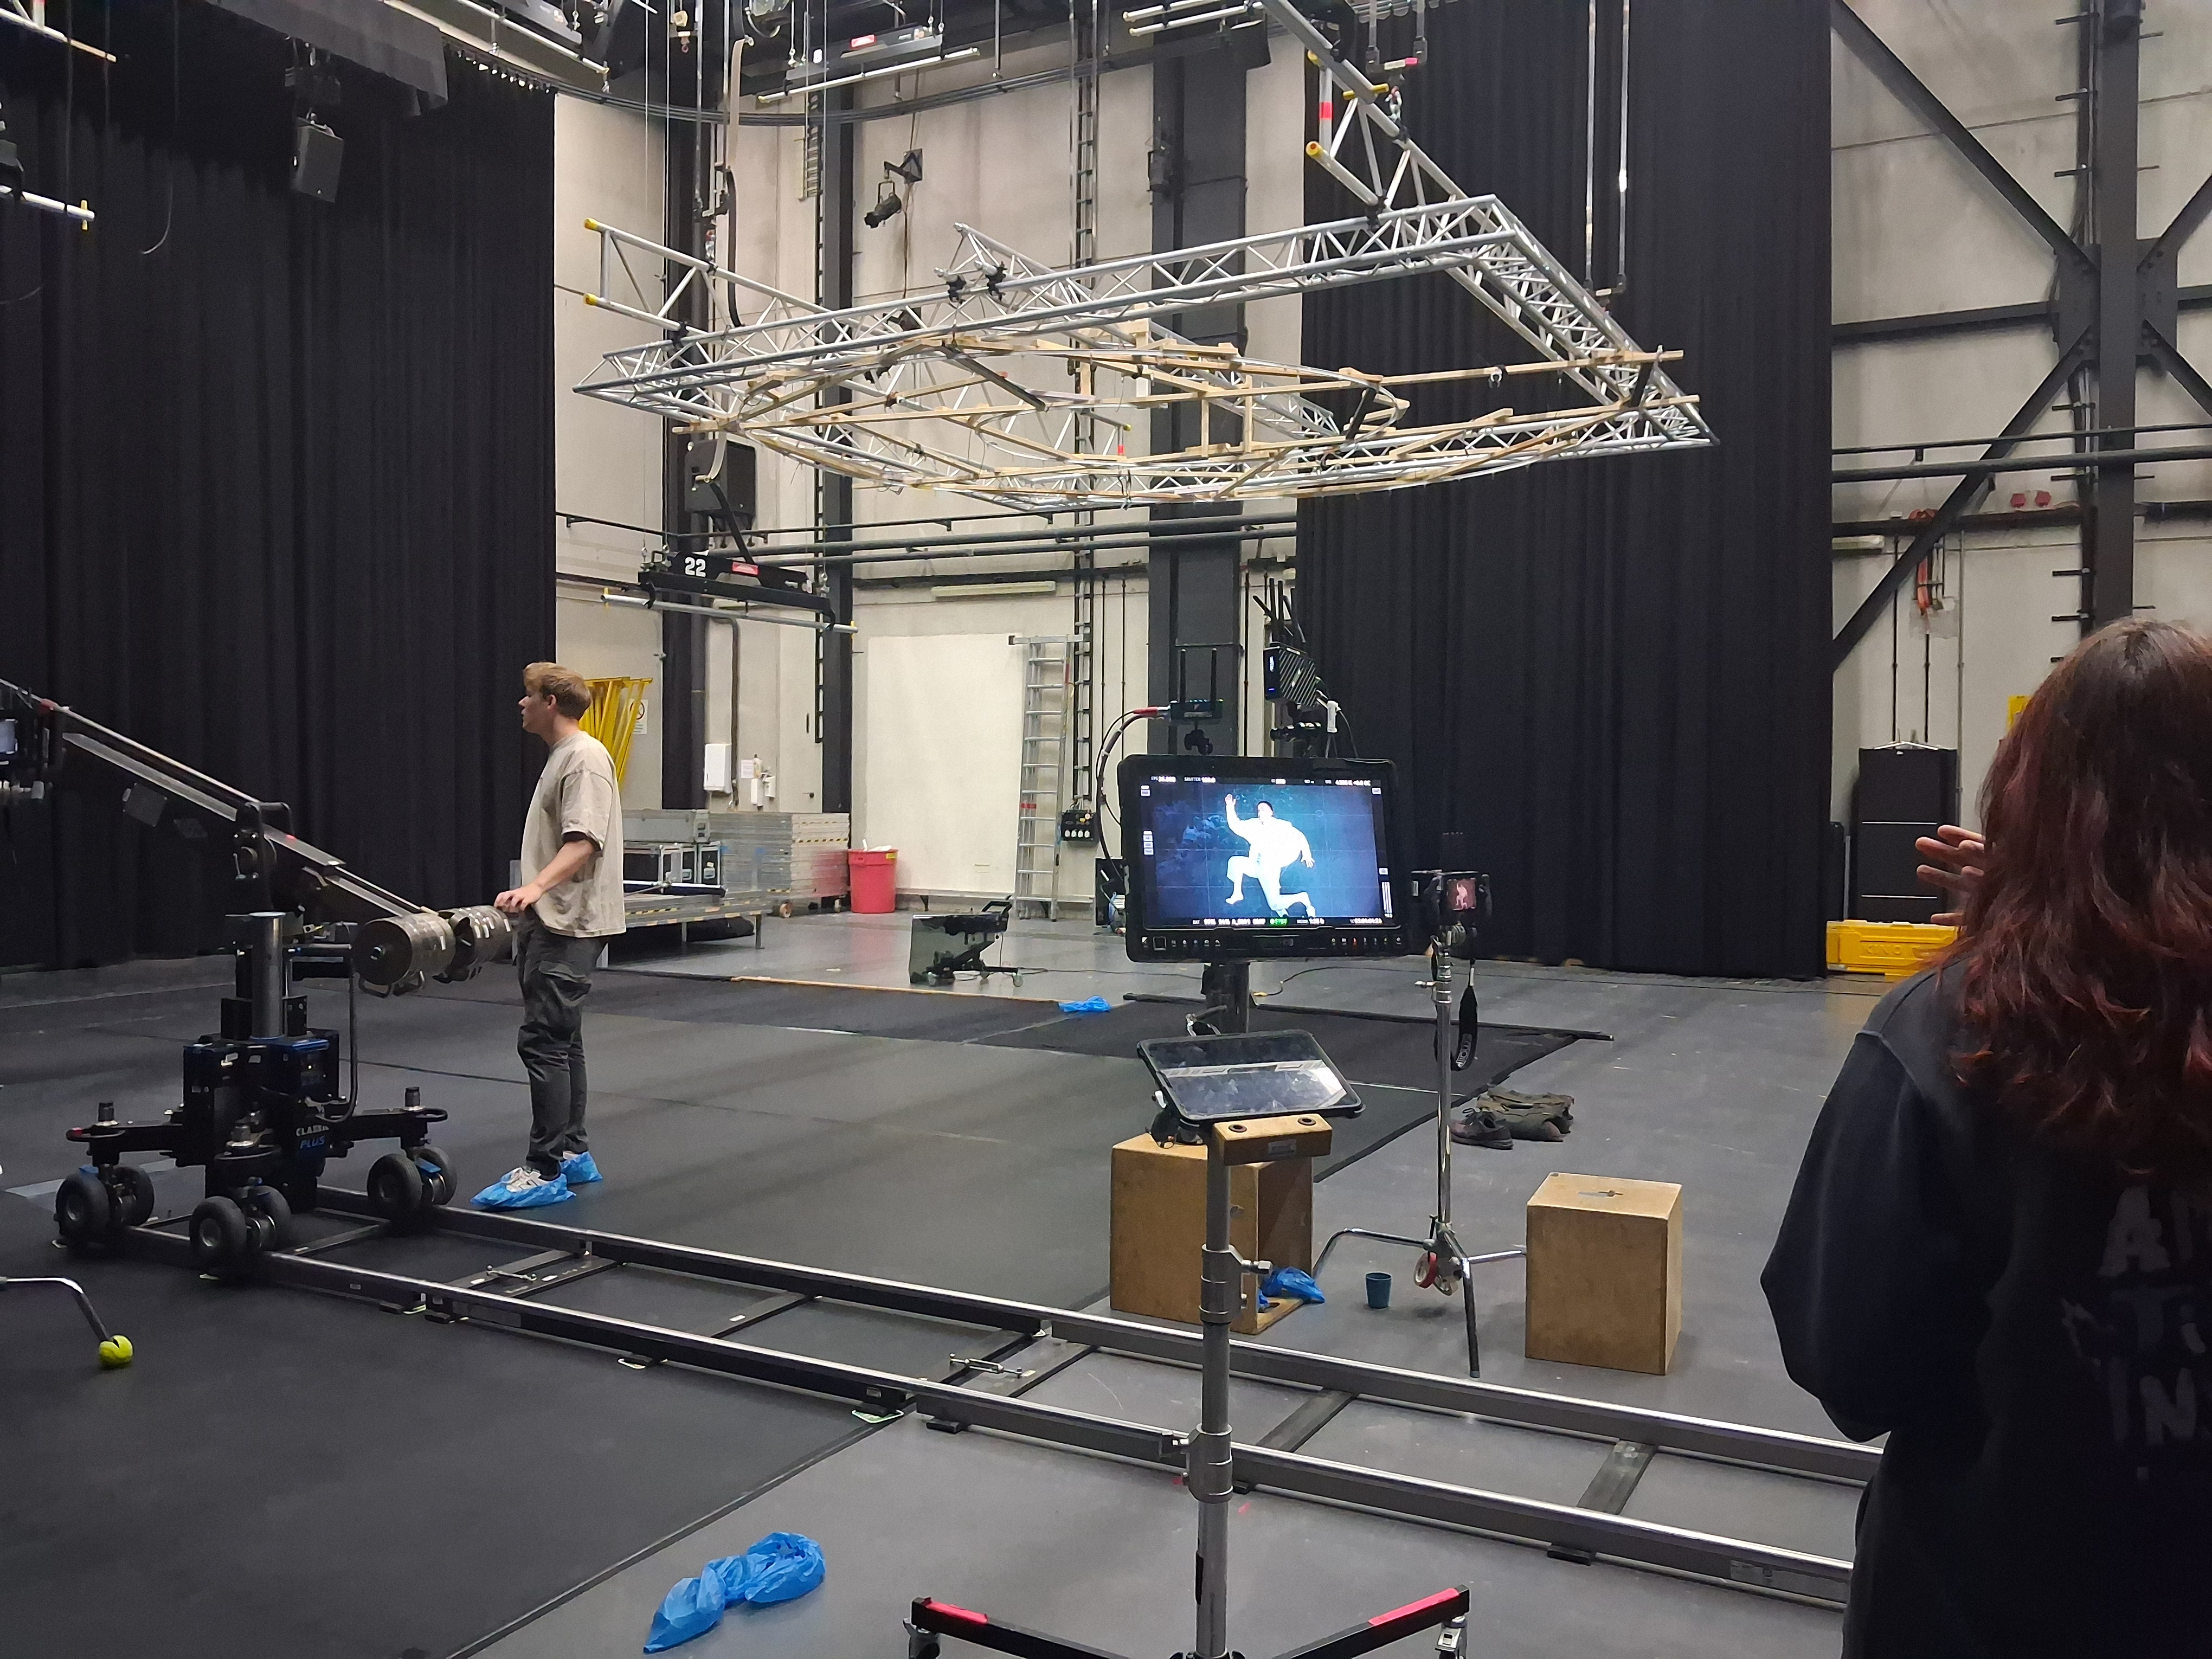
\includegraphics{images/onSetImages/cameraBTSPicofACameraScreenOfTopDown64SpikeOfDancerOnFloor.jpg}%
    }
    \caption{Kameramonitor: Top-Down-Aufnahme BTS des 64-Spike-Systems mit Tänzer auf dem Studioboden}
    \label{fig:camera_monitor}
\end{figure}

% PLACEMENT: Ausfuehrungsdokumentation.tex or ergebnisuebersicht.tex - Live system operation
\begin{figure}[htbp]
    \centering
    \adjustbox{max width=0.9\textwidth, max height=0.7\textheight, keepaspectratio}{%
        \includegraphics{images/onSetImages/BTS_ProducerScreen.png}%
    }
    \caption{Spike-System in Aktion: Reagierte präzise auf Hand- und Fußbewegungen}
    \label{fig:spike_action}
\end{figure}

% PLACEMENT: erkenntnisse.tex - Complex head-tracking setup showing technical challenges with hardcoded offsets
\FloatBarrier
\begin{figure}[htbp]
    \centering
    \adjustbox{max width=0.9\textwidth, max height=0.8\textheight, keepaspectratio}{%
        \includegraphics{images/onSetImages/HeadTracking_HQCamera.png}%
    }
    \caption{Kopfpartikel-Setup: Komplexe Kamera-Beamer-Ausrichtung mit hardcoded Offsets in particleGPU je nach Kamera-Winkel, was zu einer Erhöhung der Zeit zwischen Takes führte}
    \label{fig:head_setup}
\end{figure}

% PLACEMENT: Ausfuehrungsdokumentation.tex - Production setup challenges
\begin{figure}[htbp]
    \centering
    \adjustbox{max width=0.7\textwidth, max height=0.8\textheight, keepaspectratio}{%
        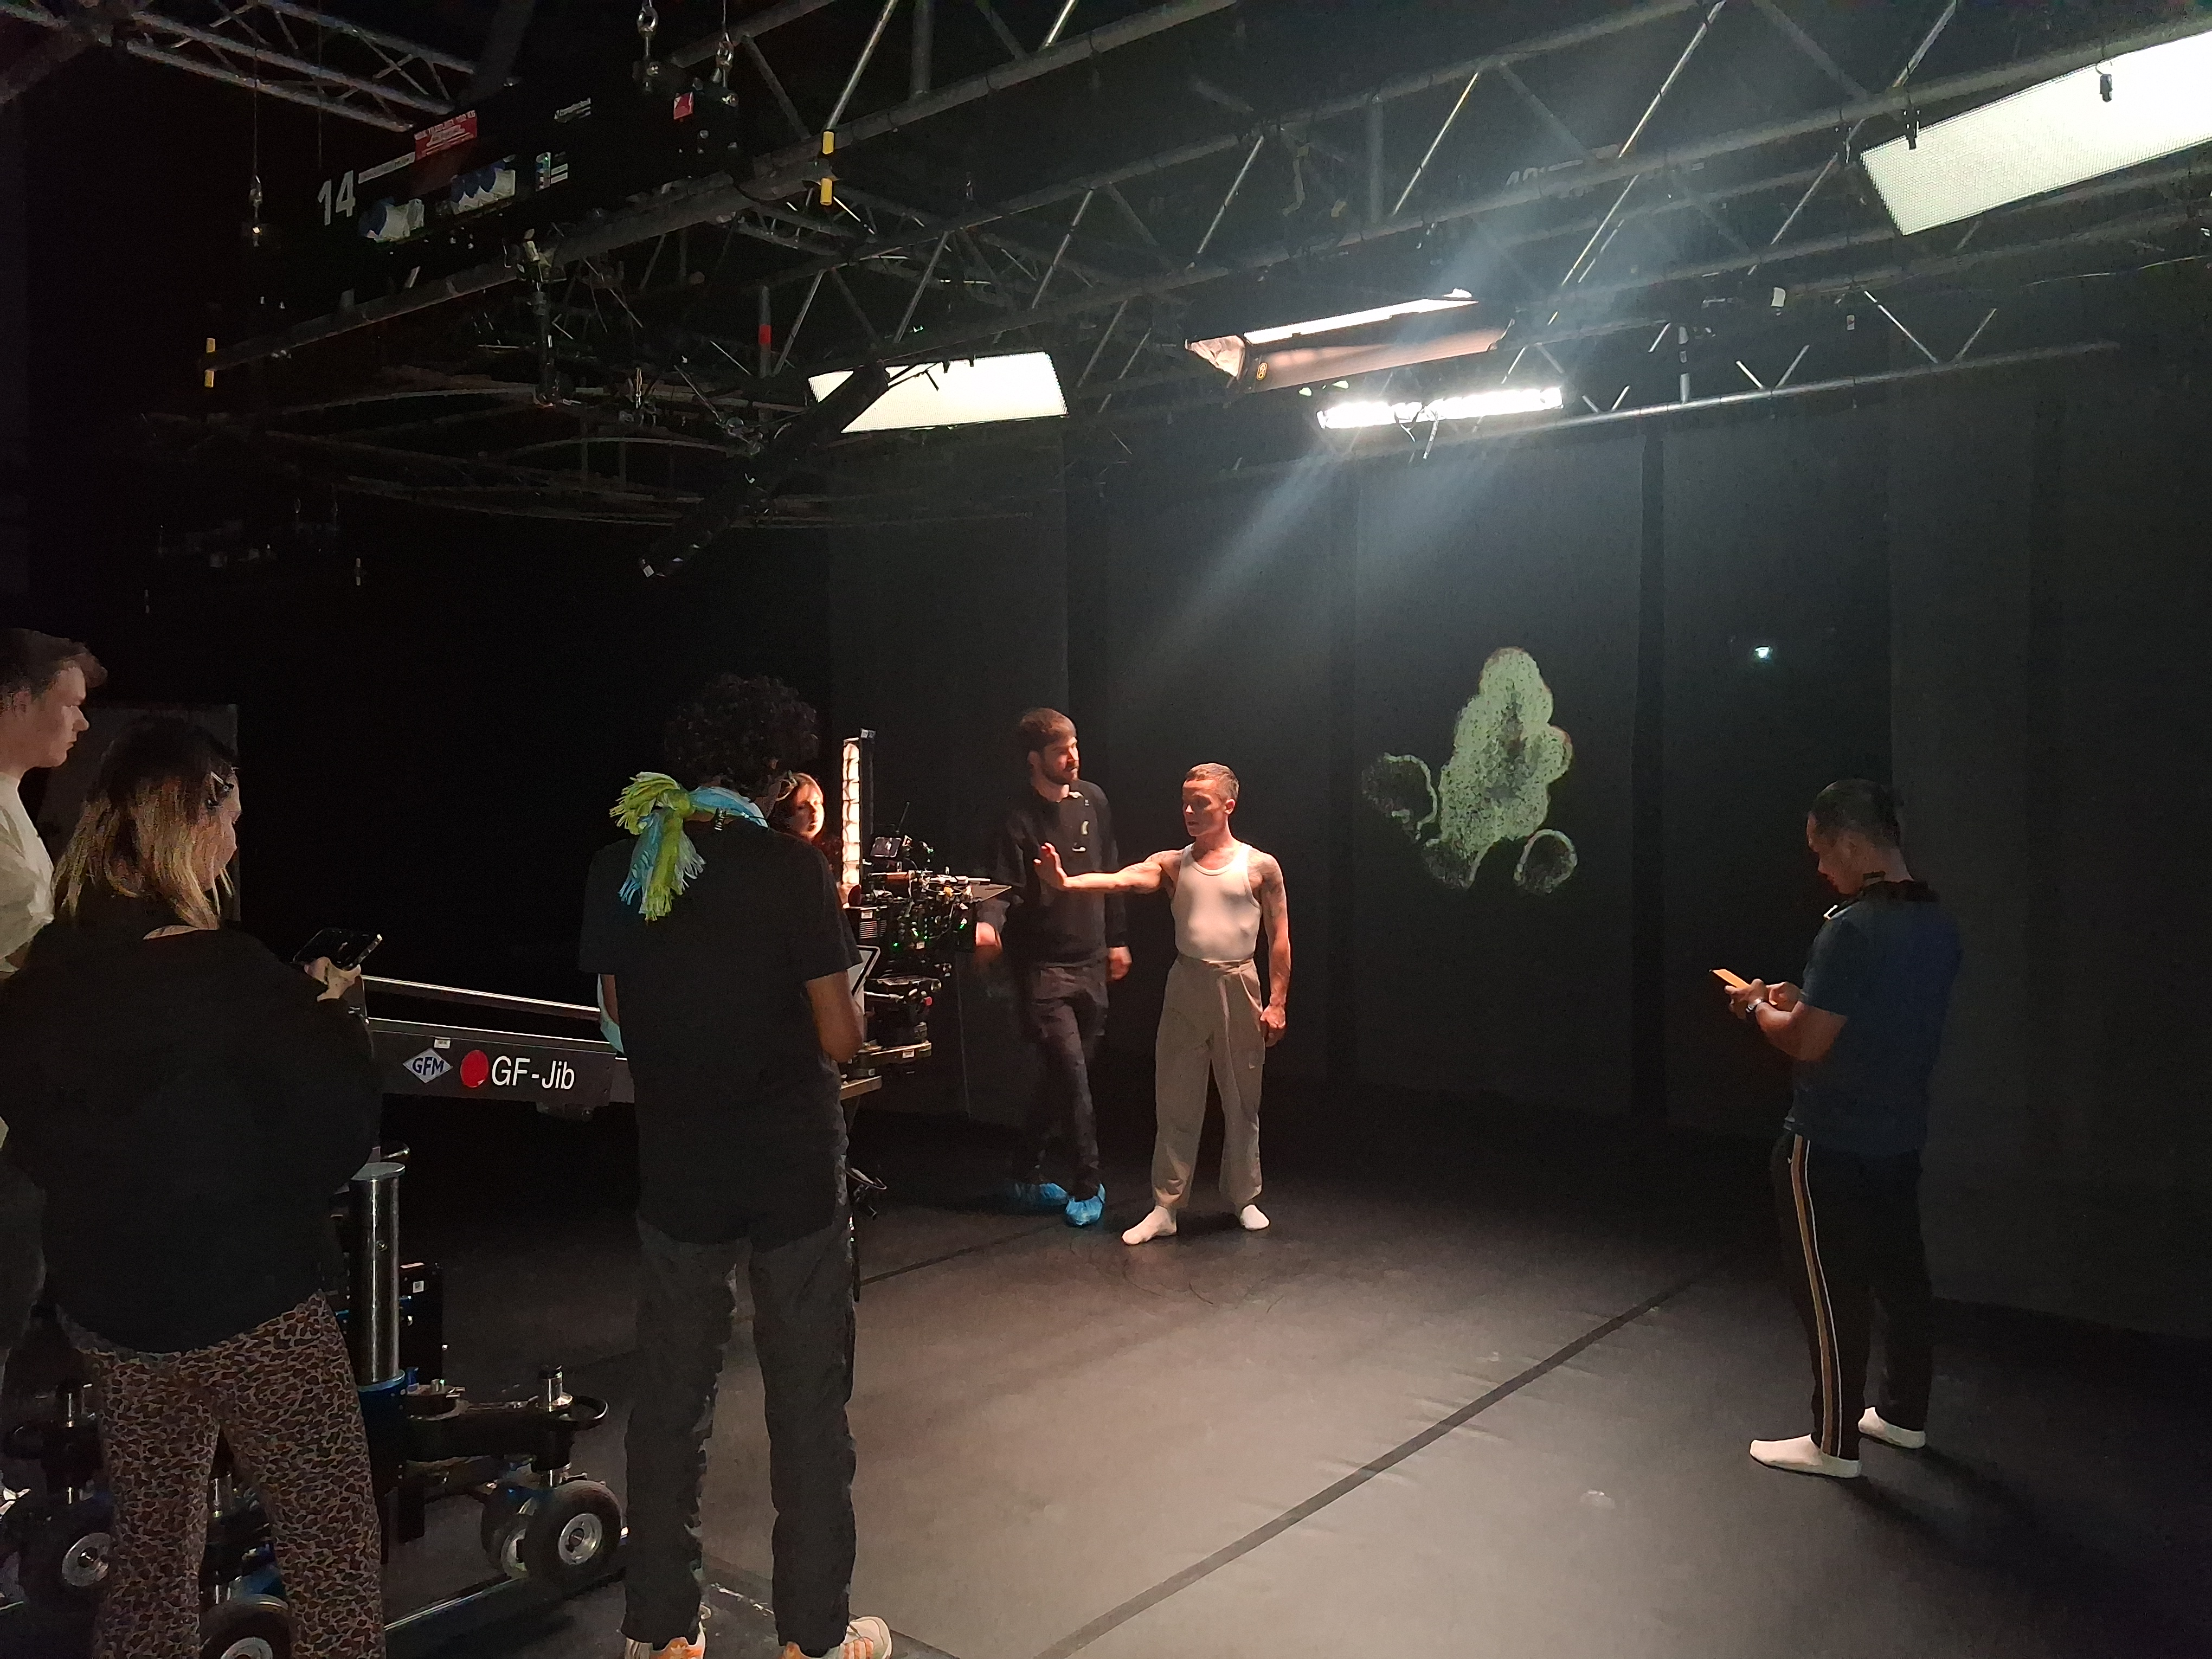
\includegraphics{images/onSetImages/PictureOfDancerBTSinSetupForHeadTrackingBubbles.jpg}%
    }
    \caption{Kopfpartikel-Setup: Tänzer bei Vorbereitung für Head-Tracking mit kritischen Lichtbedingungen. Schön zu sehen ist die Beamer-Visuals hinter Ihm.}
    \label{fig:dancer_head_tracking}
\end{figure}

% PLACEMENT: Demonstration.tex or ergebnisuebersicht.tex - Head-tracking accuracy results
\begin{figure}[htbp]
    \centering
    \adjustbox{max width=0.9\textwidth, max height=0.8\textheight, keepaspectratio}{%
        \includegraphics{images/onSetImages/HeadTrackingLeftSideOfHeadWithHeadClearlyAttached.png}%
    }
    \caption{Head-Tracking Perspektive mit seitlichem Blickwinkel. Die Blobs sind präzise am Kopf des Performers angebracht}
    \label{fig:low_light_tracking}
\end{figure}

% PLACEMENT: Demonstration.tex or ergebnisuebersicht.tex - Successful head-tracking results
\begin{figure}[htbp]
    \centering
    \adjustbox{max width=0.8\textwidth, max height=0.8\textheight, keepaspectratio}{%
        \includegraphics{images/onSetImages/HeadtrackingBubblesClearlyAtHeadLevelOnBackgroundBeamerMediaPipeSkeletonBeautifullyVisible.png}%
    }
    \caption{TouchDesigner und Kinect Perspektive: Head-Tracking-Bubbles Endergebnis: MediaPipe-Skelett-Erkennung mit Beamer-Projektion trotz Herausforderungen erfolgreich}
    \label{fig:head_result}
\end{figure}

% PLACEMENT: Demonstration.tex or ergebnisuebersicht.tex - Hand-fire effect demonstration
\begin{figure}[htbp]
    \centering
    \adjustbox{max width=0.9\textwidth, max height=0.8\textheight, keepaspectratio}{%
        \includegraphics{images/onSetImages/HQCinemaCameraPerspectiveOfHandFireToTheSidesOfTheHands.png}%
    }
    \caption{Performer hat das Hand-Feuer bei sich beim beidseitigen Anheben seiner Arme. Hier aus der Sicht der HQ-Kamera.}
    \label{fig:hand_fire_setup}
\end{figure}

% PLACEMENT: erkenntnisse.tex - Critical system limitation: tracking loss with cloth occlusion requiring manual intervention
\FloatBarrier
\begin{figure}[htbp]
    \centering
    \adjustbox{max width=0.8\textwidth, max height=0.8\textheight, keepaspectratio}{%
        \includegraphics{images/onSetImages/DancerNotMediaPipeFoundCorrectlyWhenInClothOnFloor.png}%
    }
    \caption{Tracking-Problem: MediaPipe verliert Tänzer-Skelett-Erkennung bei Stoffverschleierung zu Beginn des Visuals -> Visuals werden manuell von mir anhand der Debug-Visualisierung an und dann zum Ende ausgeschaltet, wenn Ich sah, dass der Tänzer gut erkennt wird.}
    \label{fig:cloth_tracking_issue}
\end{figure}

% PLACEMENT: Demonstration.tex or ergebnisuebersicht.tex - Live effect demonstration
\begin{figure}[htbp]
    \centering
    \adjustbox{max width=0.8\textwidth, max height=0.8\textheight, keepaspectratio}{%
        \includegraphics{images/onSetImages/dancerWithHandFireViewFromKinect.png}%
    }
    \caption{Hand-Feuer in Aktion, Sicht aus TouchDesigner: Blaue Partikel folgen den Händen. Gut zu erkennen ist das MediaPipe-Skelett, dass auch die nicht sichtbaren Füße predicted.}
    \label{fig:hand_fire_action}
\end{figure}

% PLACEMENT: Ausfuehrungsdokumentation.tex - Production conclusion
\FloatBarrier
\begin{figure}[htbp]
    \centering
    \adjustbox{max width=0.8\textwidth, max height=0.8\textheight, keepaspectratio}{%
        \includegraphics{images/onSetImages/WideShotOfOutsideOfStudioAfter2DayShoot.jpg}%
    }
    \caption{Produktionsabschluss: Außenansicht des Albrecht-Ade-Studios nach zweitägiger Drehzeit}
    \label{fig:studio_exterior}
\end{figure}

% PLACEMENT: Ausfuehrungsdokumentation.tex - Team dynamics and production atmosphere
\begin{figure}[htbp]
    \centering
    \adjustbox{max width=0.9\textwidth, max height=0.6\textheight, keepaspectratio}{%
        \includegraphics{images/onSetImages/MartySmileyIntoCameraOnSet.jpg}%
    }
    \caption{Teamdynamik: Entspannte Atmosphäre zwischen den Takes trotz technischer Herausforderungen}
    \label{fig:team_atmosphere}
\end{figure}

% PLACEMENT: Top-Down-Shot!!! GUTES BILD DAFÜR!!!
\begin{figure}[htbp]
    \centering
    \adjustbox{max width=0.8\textwidth, max height=0.8\textheight, keepaspectratio}{%
        \includegraphics{images/onSetImages/BTS_TopDown_DancerAndProducer.png}%
    }
    \caption{Behind the Scenes: Tänzer mit professioneller Lichttechnik und Producer-Ansicht beim Top-Down-Shot}
    \label{fig:studio_wide}
\end{figure}

% ===== Visual-Effekt-Demonstrationen =====
% Für Abschnitt: Demonstration oder Systemarchitektur
\FloatBarrier

% PLACEMENT: Demonstration.tex or ergebnisuebersicht.tex - Key visual effect demonstration
\begin{figure}[htbp]
    \centering
    \adjustbox{max width=0.8\textwidth, max height=0.8\textheight, keepaspectratio}{%
        \includegraphics{images/docupictures/DemonstrationOfTheMagicalFireHands.png}%
    }
    \caption{Live-Demonstration des NoisyBlob Hand-Feuer-Effekts bei mir im Test-Setup zuhause: Blaue Partikel-Emission folgen den Händen}
    \label{fig:handfeuer_demonstration}
\end{figure}

% ===== Head-Tracking-System Ansichten =====
% Für Abschnitt: Systemarchitektur oder Demonstration
\FloatBarrier

% PLACEMENT: Demonstration.tex or Systemarchitektur_und_Ergebnisse.tex - Precise tracking demonstration
\begin{figure}[htbp]
    \centering
    \adjustbox{max width=0.9\textwidth, max height=0.8\textheight, keepaspectratio}{%
        \includegraphics{images/onSetImages/HQCameraHeadtrackingVisibleWithBubblesOffsetCorrectlyFromHQCameraViewToAppearOnRightSideOfHead.png}%
    }
    \caption{HQ-Kameraperspektive: Kopfpartikel mit korrektem Offset zur rechten Seite des Performers für präzise Beamer-Projektion}
    \label{fig:headtracking_hq_kamera_offset}
\end{figure}

% PLACEMENT: Systemarchitektur_und_Ergebnisse.tex or anhang_technische_spezifikationen.tex - Technical debugging visualization
\begin{figure}[htbp]
    \centering
    \adjustbox{max width=0.8\textwidth, max height=0.8\textheight, keepaspectratio}{%
        \includegraphics{images/onSetImages/HeadTrackingPerspectiveTouchDesignerWithVisualsOverlayedAboveDebugCompToSeeaccurateTrackingOfParticleGPUaboveHeadWithReallifeBeamerProjectionCorrectlyPlaced.png}%
    }
    \caption{Debug-Visualisierung: Präzises ParticleGPU-Tracking über Kopfposition mit korrekt ausgerichteter Beamer-Projektion}
    \label{fig:headtracking_debug_overlay}
\end{figure}

% PLACEMENT: erkenntnisse.tex or Systemarchitektur_und_Ergebnisse.tex - Technical challenges and solutions
\begin{figure}[htbp]
    \centering
    \adjustbox{max width=0.8\textwidth, max height=0.8\textheight, keepaspectratio}{%
        \includegraphics{images/onSetImages/HeadTrackedBubblesInActionTouchDesignerPerspectiveslightMediaPipeFrameDelaySeeableButAlsoVisualsDirectlyAtHead.png}%
    }
    \caption{TouchDesigner Head-Tracking in Aktion: Kopfpartikel-Bubbles mit sichtbarer MediaPipe-Frame-Verzögerung aber direkter visueller Kopfanbindung}
    \label{fig:headtracking_bubbles_aktion}
\end{figure}

% ===== Technische Implementierung =====
% Für Abschnitt: Entwicklungsprozess oder Systemarchitektur
\FloatBarrier

% PLACEMENT: Systemarchitektur_und_Ergebnisse.tex - Key innovation: Infrared pipeline for production lighting conditions
\begin{figure}[htbp]
    \centering
    \adjustbox{max width=0.8\textwidth, max height=0.8\textheight, keepaspectratio}{%
        \includegraphics{images/docupictures/InfraRedOBSCameraToMediaPipeForTopDownCirlceGradeMapping.png}%
    }
    \caption{Infrarot-Pipeline im Test zuhause: Kinect V2 IR-Stream über OBS Virtual Camera zu MediaPipe für störungsfreies Top-Down-Tracking}
    \label{fig:infrarot_topdown_mapping}
\end{figure}

% PLACEMENT: Systemarchitektur_und_Ergebnisse.tex or anhang_technische_spezifikationen.tex - Complete system architecture
\begin{figure}[htbp]
    \centering
    \adjustbox{max width=0.9\textwidth, max height=0.8\textheight, keepaspectratio}{%
        \includegraphics{images/docupictures/Finished_MediaPipeContainer.png}%
    }
    \caption{Vollständiger MediaPipe-Integration-Container ohne Erklärungen: Modulare Node-Netzwerk-Architektur für Skelett-Tracking-Datenverarbeitung}
    \label{fig:mediapipe_container_komplett}
\end{figure}